\iffalse
\let\negmedspace\undefined
\let\negthickspace\undefined
\documentclass[journal,12pt,onecolumn]{IEEEtran}

\usepackage{cite}
\usepackage{amsmath,amssymb,amsfonts,amsthm}
\usepackage{algorithmic}
\usepackage{graphicx}
\usepackage{textcomp}
\usepackage{xcolor}
\usepackage{txfonts}
\usepackage{listings}
\usepackage{enumitem}
\usepackage{mathtools}
\usepackage{gensymb}
\usepackage[breaklinks=true]{hyperref}
\usepackage{tkz-euclide} % loads  TikZ and tkz-base
\usepackage{listings}
\usepackage{circuitikz}
\usepackage{graphicx}

%\newcounter{MYtempeqncnt}
\DeclareMathOperator*{\Res}{Res}
%\renewcommand{\baselinestretch}{2}
\renewcommand\thesection{\arabic{section}}
\renewcommand\thesubsection{\thesection.\arabic{subsection}}
\renewcommand\thesubsubsection{\thesubsection.\arabic{subsubsection}}

\renewcommand\thesectiondis{\arabic{section}}
\renewcommand\thesubsectiondis{\thesectiondis.\arabic{subsection}}
\renewcommand\thesubsubsectiondis{\thesubsectiondis.\arabic{subsubsection}}

% correct bad hyphenation here
\hyphenation{op-tical net-works semi-conduc-tor}
\def\inputGnumericTable{}                                 %%

\lstset{
	frame=single,
	breaklines=true,
	columns=fullflexible
}

\newtheorem{theorem}{Theorem}[section]
\newtheorem{problem}{Problem}
\newtheorem{proposition}{Proposition}[section]
\newtheorem{lemma}{Lemma}[section]
\newtheorem{corollary}[theorem]{Corollary}
\newtheorem{example}{Example}[section]
\newtheorem{definition}[problem]{Definition}
\newcommand{\BEQA}{\begin{eqnarray}}
	\newcommand{\EEQA}{\end{eqnarray}}
\newcommand{\define}{\stackrel{\triangle}{=}}
\newcommand\figref{Fig.~\ref}
\newcommand\tabref{Table~\ref}
\bibliographystyle{IEEEtran}
%\bibliographystyle{ieeetr}


\providecommand{\mbf}{\mathbf}
\providecommand{\pr}[1]{\ensuremath{\Pr\left(#1\right)}}
\providecommand{\qfunc}[1]{\ensuremath{Q\left(#1\right)}}
\providecommand{\sbrak}[1]{\ensuremath{{}\left[#1\right]}}
\providecommand{\lsbrak}[1]{\ensuremath{{}\left[#1\right.}}
\providecommand{\rsbrak}[1]{\ensuremath{{}\left.#1\right]}}
\providecommand{\brak}[1]{\ensuremath{\left(#1\right)}}
\providecommand{\lbrak}[1]{\ensuremath{\left(#1\right.}}
\providecommand{\rbrak}[1]{\ensuremath{\left.#1\right)}}
\providecommand{\cbrak}[1]{\ensuremath{\left\{#1\right\}}}
\providecommand{\lcbrak}[1]{\ensuremath{\left\{#1\right.}}
\providecommand{\rcbrak}[1]{\ensuremath{\left.#1\right\}}}
\theoremstyle{remark}
\newtheorem{rem}{Remark}
\newcommand{\sgn}{\mathop{\mathrm{sgn}}}
\providecommand{\abs}[1]{\left\vert#1\right\vert}
\providecommand{\res}[1]{\Res\displaylimits_{#1}}
\providecommand{\norm}[1]{\left\lVert#1\right\rVert}
%\providecommand{\norm}[1]{\lVert#1\rVert}
\providecommand{\mtx}[1]{\mathbf{#1}}
\providecommand{\mean}[1]{E\left[ #1 \right]}
\providecommand{\fourier}{\overset{\mathcal{F}}{ \rightleftharpoons}}
%\providecommand{\hilbert}{\overset{\mathcal{H}}{ \rightleftharpoons}}
\providecommand{\system}{\overset{\mathcal{H}}{ \longleftrightarrow}}
%\newcommand{\solution}[2]{\textbf{Solution:}{#1}}
\newcommand{\solution}{\noindent \textbf{Solution: }}
\newcommand{\cosec}{\,\text{cosec}\,}
\providecommand{\dec}[2]{\ensuremath{\overset{#1}{\underset{#2}{\gtrless}}}}
\newcommand{\myvec}[1]{\ensuremath{\begin{pmatrix}#1\end{pmatrix}}}
\newcommand{\mydet}[1]{\ensuremath{\begin{vmatrix}#1\end{vmatrix}}}
\renewcommand{\abstractname}{Question}

\let\vec\mathbf


	

\newcommand{\permcomb}[4][0mu]{{{}^{#3}\mkern#1#2_{#4}}}
\newcommand{\comb}[1][-1mu]{\permcomb[#1]{C}}

%\IEEEpeerreviewmaketitle

\newcommand \tab [1][1cm]{\hspace*{#1}}
%\newcommand{\Var}{$\sigma ^2$}
\usepackage{amssymb}
\usepackage{amsmath}
\title{
	
\title{NCERT Physics 12.7 Q19}
\author{EE23BTECH11212 - MANUGUNTA MEGHANA SAI$^{*}$% <-this % stops a space
}


}
\begin{document}

\maketitle

\textbf{Question:} 
A circuit containing a $80 mH$ inductor and a $60 \mu F$ capacitor in series is connected to a $230 V$, $50 Hz$ supply. A resistance of $15 \Omega $ is connected in series. Obtain the average power transferred to each element of the circuit, and the total power absorbed.\\
\\

\solution
\fi
\begin{figure}[h]
	\centering
	    %\begin{circuitikz}
		% Draw the components
	%	\draw (0,0) to[V, v=$230\,V$, f=$50\,Hz$] (0,3)
	%	to[R, l=$15\,\Omega$] (3,3)
	%	to[L, l=$80\,mH$] (6,3)
	%	to[C, l=$60\,\mu F$] (6,0)
	%	-- (0,0);
    % \end{circuitikz}
\begin{circuitikz}
	\draw(0, 0) -- (1, 0);
	\draw(1, 0) to [L, l = $80\,mH$](2, 0);
	\draw(2, 0) -- (3, 0);
	\draw(3, 0) to [C, l = $60\,\mu F$](4, 0);
	\draw(4, 0) -- (5, 0);
	\draw(5, 0) to [R, l = $15\,\Omega$](6, 0);
	\draw(0, 0) -- (0, -2);
	\draw[->] (0, -1) node[left] {$I(s)$} -- (0, -1);
	\draw(6, 0) -- (7, 0);
	\draw(7, 0) -- (7, -2);
	\draw(0, -2) -- (3, -2);
	\draw(7, -2) -- (7, -2);
	\draw(3, -2) to [sV, l = $230\,V$](4, -2);
	\draw(4, -2) -- (7, -2);
\end{circuitikz}


	\caption{LCR Circuit}
	\label{fig:msm11.7.19fig2}
\end{figure}
     
In~\figref{fig:msm11.7.19fig2} the following information is provided:
 
 

 \begin{table}[h!]
 	\centering
 	\resizebox{6 cm}{!}{
 		\begin{tabular}{|c|c|c|}
	\hline
	\textbf{Symbol} & \textbf{Value} &
	\textbf{Description}\\[6pt]
	\hline
	$L$ &  $80mH$ & Inductance\\[6pt]
	\hline 
	$C$ &  $60\, \mu F$ & Capacitance \\[6pt]
	\hline
	$R$ &  $15\, \Omega$ & Resistance\\[6pt]
	\hline
	$V_{rms}$ & $230\, V$ & Voltage\\[6pt]
	\hline
	$f$ & $50\, {Hz}$ & Frequency\\[6pt]
	\hline
	$\omega$ & $2\pi f=100\pi$ & Angular Frequency\\[6pt]
	\hline
	$\phi$ & $-$ & Phase difference between current and voltage\\[6pt]
	\hline
	$I_ \text{rms}$ & $-$ & rms value of current\\
	\hline
	$V_m$ & $-$ & Maximum voltage\\
	\hline
	$I_m$ & $-$ & Maximum current\\
	\hline
	$P_m$ & $-$ & Maximum Power\\
	\hline
\end{tabular}

 	}
 	\caption{Given Parameters}
 	\label{tab:msm11.7.19tab1} 
 \end{table} 
 \text{Applying Kirchoff's Voltage Law} in the~\figref{fig:msm11.7.19fig1}
 
 \begin{figure}[!h]
 	\centering
 	\begin{circuitikz}
	\draw(0, 0) -- (1, 0);
	\draw(1, 0) to [L, l = $sL$](2, 0);
	\draw(2, 0) -- (3, 0);
	\draw(3, 0) to [C, l = $\frac{1}{sC}$](4, 0);
	\draw(4, 0) -- (5, 0);
	\draw(5, 0) to [R, l = $R$](6, 0);
	\draw(0, 0) -- (0, -2);
	\draw[->] (0, -1) node[left] {$I(s)$} -- (0, -1);
	\draw(6, 0) -- (7, 0);
	\draw(7, 0) -- (7, -2);
	\draw(0, -2) -- (3, -2);
	\draw(7, -2) -- (7, -2);
	\draw(3, -2) to [sV, l = $V(s)$](4, -2);
	\draw(4, -2) -- (7, -2);
\end{circuitikz}
 	\caption{s domain circuit}
 	\label{fig:msm11.7.19fig1}
 	
 \end{figure}
 \begin{align}
 	V(s) &= R I(s) + sL I(s) + \dfrac{1}{sC} I(s)\\
         &= I(s)\left(R + sL + \dfrac{1}{sC}\right)
 \end{align}
\begin{align}
    I(s) &= \dfrac{V(s)}{\left(R + sL + \dfrac{1}{sC}\right)}\\ 
    H(s) &= \dfrac{V(s)}{I(s)}\\
	H(s) &= R + sL + \dfrac{1}{sC}
\end{align}

Substituting $s$ with $j \omega$
\begin{align}
	H(j\omega) = R + j\omega L + \dfrac{1}{j\omega C}
\end{align}
\begin{align}
	\Rightarrow \lvert H(j\omega) \rvert = \sqrt{R^2 + \left(\omega L - \dfrac{1}{\omega C}\right)^2}
\end{align}
Let the input voltage be:
\begin{align}
	V=V_{m}sin\brak{\omega t}
\end{align}
Let the current at a given instant be:
\begin{align}
	I=I_{m}sin\brak{\omega t - \phi}
\end{align}
Instantaneous power is given by:
\begin{align}
	P &= VI\\
	P &= V_{m}sin\brak{\omega t} \times I_{m}sin\brak{\omega t - \phi}
\end{align}
Average power is given by:
\begin{align}
	P_{av} &= \frac{W}{T}\\
	dW &= Pdt
\end{align}
Integrating on both sides 
\begin{align}
	W &= V_{m}I_{m} \int_{0}^{T} \sin\brak{\omega t} \sin\brak{\omega t - \phi} \, dt \\
	&= V_{m}I_{m} \int_{0}^{T} \sin\brak{\omega t}\brak{\sin(\omega t)\cos(\phi) - \cos(\omega t)\sin(\phi)} \, dt \\
	&= V_{m}I_{m} \int_{0}^{T} (\sin(\omega t))^2\cos(\phi) \, dt - V_{m}I_{m} \int_{0}^{T} \sin(\omega t)\cos(\omega t)\sin(\phi) \, dt \\
	&= V_{m}I_{m} \int_{0}^{T} \frac{1 - \cos(2\omega t)}{2}\cos(\phi) \, dt - V_{m}I_{m} \int_{0}^{T} \sin(2\omega t)\sin(\phi) \, dt
\end{align}
After solving the integral we get,
\begin{align}
	W=\frac{1}{2}V_{m}I_{m}Tcos{\phi}
\end{align}
Relation between $V_{rms}$ and $V_m$:
\begin{align}
	V_{\text{rms}} &= \frac{V_{m}}{\sqrt{2}}
\end{align}	
Relation between $I_{rms}$ and $I_m$:
\begin{align}
	I_{\text{rms}} &= \frac{I_{m}}{\sqrt{2}}
\end{align}
a) The average power dissipated in a RLC circuit is given by :
\begin{equation}
	P=V_{rms} I_{rms} cos(\phi) 
	\label{eq:msm11.7.19eq1}
\end{equation}
The phase difference is given by:
\begin{align}
	tan\brak{\phi} = \frac{\frac{1}{\omega C}-\omega L}{R}
\end{align}
After substituting the values from~\tabref{tab:msm11.7.19tab1}:
\begin{align}
	tan\brak{\phi} = 1.86
\end{align}

Rms value of current $I_{rms}$ is given by  :
\begin{align}
	I_{rms}=\frac{V_{rms}}{R}=\frac{230}{15}=15.33A
\end{align}
Now, susbtituting the value of $\phi$, $I_{rms}$ and values from~\tabref{tab:msm11.7.19tab1} in~\eqref{eq:msm11.7.19eq1} we obtain the total power :
\begin{align}
	P_{av}=789.62 W
\end{align}
b) Average power transferred to the capacitor, $P_C$:\\
For a capacitor the phase angle is:
\begin{align}
	\phi &= \frac{\pi}{2}\\
	cos(\phi) &= 0\\
	P_C &= 0
\end{align}	  

c) Average power transferred to the inductor, $P_L$:\\
For an inductor the phase angle is:
\begin{align}
	\phi &= -\frac{\pi}{2}\\
	cos(\phi) &= 0\\
	P_L &= 0
\end{align}	 

d) Average Power transferred to the resistor, $P_R$:

\begin{align}
	P_{avg} &= P_{R} + P_{C} + P_{L}\\
	P_{R} &= P_{avg} - P_{C} - P_{L}\\
	P_{R} &= 789.62 -0-0\\
	P_R &= 789.62W
\end{align}

\newpage
\begin{figure}[!h]
	\centering
	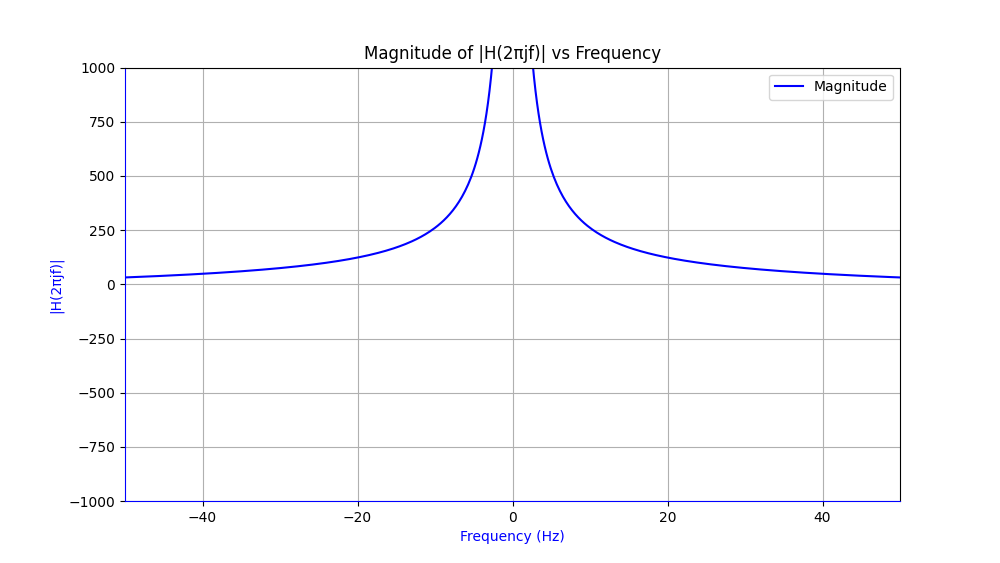
\includegraphics[width=\columnwidth]{ncert-physics/12/7/19/figs/rmagnitude.png}
	\caption{$\abs{H(j/omega)}$ vs $\omega$}
\end{figure}

Bandwidth is defined as the range of frequencies, where power ranges from its maximium value to half of its maximum value.

\begin{align}
I_{rms} = \frac{V_{rms}}{\abs{H\brak{j\omega}}}      
\end{align}
At maximum power, $\abs{H\brak{j\omega}}$ will be minimum,
\begin{align}
\abs{H\brak{j\omega}} = R\\
I_{m} = \frac{V_{rms}}{R}
\end{align}
when, power is half of the maximum value of power
\begin{align}
P &= \frac{P_{m}}{2}\\
I_{rms} &= \frac{I_{m}}{\sqrt{2}}\\
\abs{H\brak{j\omega}}&=\sqrt{2}R\\
\sqrt{R^2 + \left(\omega L - \dfrac{1}{\omega C}\right)^2} &= \sqrt{2} R\\
\left(\omega L - \dfrac{1}{\omega C}\right)^2 &= R^{2}
\end{align}
This equation has 2 roots, $\omega_{1}$ and $\omega_{2}$:
\begin{align}
\omega_{1} &= -\frac{R}{2L} + \sqrt{\frac{R^{2}}{4R}+\frac{1}{LC}}\\
\omega_{2} &= \frac{R}{2L} + \sqrt{\frac{R^{2}}{4R}+\frac{1}{LC}}
\end{align}
Thus Bandwidth of circuit is :
\begin{align}
\omega_{2}-\omega_{1} = \frac{R}{L} = 187.5\\
f = \frac{\omega_{2}-\omega_{1}}{2\pi} = 29.85 
\end{align}

%\end{document}

